\documentclass{standalone}
\usepackage{pgfplots}
\pgfplotsset{compat=newest}

\usepackage{tikz}


\usetikzlibrary{shapes.geometric, arrows, positioning, angles, quotes}
\usetikzlibrary{patterns}
\usetikzlibrary{decorations.pathmorphing}
\usetikzlibrary{fit,calc}
\usetikzlibrary{snakes}

\tikzset{
	arrow/.style={-latex},
	>=latex
}

\tikzstyle{vertex} = [circle, draw=black, thick, minimum height=1.5em, text centered]
\tikzstyle{solid} = =[circle, fill,inner sep=1.5pt,outer sep=0pt]


%---------------------------------------------------------------------------------------
%   VARIABLE MAKROS
%---------------------------------------------------------------------------------------

% Solution Curve
% -> Parameter of the solution curve
\newcommand{\sCurveP}{\lambda}
% -> Region/Breakpoint index of the solution curve
\newcommand{\sCurveI}{i}
% -> Breakpoints of the solution curve
\newcommand{\sCurveB}{\lambda}
% -> Number of breakpoints of the solution curve
\newcommand{\sCurveNB}{I}

% Graph Matrices
\newcommand{\incidenceMatrix}{\vec \Gamma}
\newcommand{\incidenceM}{\incidenceMatrix}
\newcommand{\incidenceV}{\vec{\gamma}}
\newcommand{\incidenceVs}{\hat{\vec{\gamma}}}
\newcommand{\edgePathMatrix}{\vec B}

% Commodities
\newcommand{\commodity}{j}
\newcommand{\numCommodities}{k}
\newcommand{\setCommodities}{K}

% Source/Sink
\newcommand{\source}{s}
\newcommand{\sink}{t}


% Vertex related Variables
\newcommand{\vertex}{v}
\newcommand{\numVertices}{n}
\newcommand{\setVertices}{V}

% Edge related Variables
\newcommand{\edge}{e}
\newcommand{\altEdge}{{e'}}
\newcommand{\numEdges}{m}
\newcommand{\setEdges}{E}

% Active, Inactive, Used Edges
\newcommand{\activeEdges}[1][j]{\setEdges^{\mathrm{A}}_{#1}}
\newcommand{\uActiveEdges}[1][j]{\setEdges^{\mathrm{A}^+}_{#1}}
\newcommand{\lActiveEdges}[1][j]{\setEdges^{\mathrm{A}^-}_{#1}}
\newcommand{\inactiveEdges}[1][j]{\setEdges^{\mathrm{I}}_{#1}}
\newcommand{\usedEdges}[1][j]{\setEdges^{\mathrm{U}}_{#1}}

% Path related Variables
\newcommand{\pathVar}{P}
\newcommand{\altPath}{Q}
\newcommand{\setPaths}{\mathcal{P}}

% Multi commodity flow vector / variable
\newcommand{\mcFlowVec}{\vec X}
\newcommand{\mcFlow}[1][\edge, \commodity]{x_{#1}}
\newcommand{\mcPathFlow}{\bar{x}_{\path, \commodity}}
% Flow of one commodity of a multi commodity flow
\newcommand{\cFlowVec}[1][\commodity]{\vec x_{#1}}
\newcommand{\cPathFlowVec}[1][\commodity]{\bar{\vec x}^{#1}}
% Flow on one edge of a multi commodity flow
\newcommand{\mcEdgeFlow}{\vec x}
% Total flow vector
\newcommand{\totalFlow}{z}
\newcommand{\totalFlowVec}{\vec z}

% Indicator vectors / Identifier 
\newcommand{\indicatorMatrix}[1][]{
	\ifthenelse { \equal{#1}{} } 
	{	\vec{I}		}
	{	\vec{I}_{#1}	}
}
\newcommand{\idUnused}{\text{un}}
\newcommand{\idInactive}{\text{in}}
\newcommand{\idActive}{\text{ac}}
\newcommand{\indicUnused}{\vec{I}_{\commodity, \idUnused}}
\newcommand{\indicInactive}{\vec{I}^{\mathrm{I}}_{\commodity}}
\newcommand{\indicUActive}{\vec{I}^{\mathrm{A}^+}_{\commodity}}
\newcommand{\indicLActive}{\vec{I}^{\mathrm{A}^-}_{\commodity}}

% Demand
\newcommand{\demandVec}{\vec q}
\newcommand{\demand}{q}

% Region Vector
\newcommand{\regionI}{t}
\newcommand{\regionVec}{\vec{\regionI}}
\newcommand{\regionV}{\regionVec}

% Potential Space
\newcommand{\potentialSpace}{\Pi}
\newcommand{\feasiblePotentials}[1][\regionV]{\Pi_{#1}}

% Potential Region
\newcommand{\region}[1][\regionV]{R_{#1}}
\newcommand{\neighboringR}{\mathfrak{N}}

\newcommand{\regionOffset}[1][\regionV]{\vec{\pi}_{#1}}

% Coefficent Matrices
\newcommand{\aM}{\vec{A}}
\newcommand{\cM}{\vec{C}}

% Potential Vector
\newcommand{\potentialV}{\vec{\pi}}
\makeatletter
\newcommand{\potentialD}[1][\regionV]{\@ifstar{\Delta \potentialV}{\Delta \potentialV_{#1}}}
\makeatother

% Flow Vector
\newcommand{\flowV}{\vec{x}}
\newcommand{\flow}{x}

% Edge Flow Capacities
\makeatletter
\newcommand{\lcap}[1][e]{\@ifstar{l}{l_{#1}}}
\newcommand{\lcapV}{\vec{\lcap*}}
\newcommand{\ucap}[1][e]{\@ifstar{u}{u_{#1}}}
\newcommand{\ucapV}{\vec{\ucap*}}
\makeatother

% Induced Flow Vector Function
\newcommand{\inducedFlow}{\vec{\charf}^{-1}}

% Electrical characteristic function
\newcommand{\charf}{f}

% Edge cost function
\makeatletter
\newcommand{\ecost}[1][e]{\@ifstar{F}{F_{#1}}}
\newcommand{\dcost}[1][e]{\@ifstar{f}{f_{#1}}}
\makeatother

% ExcessVector
\newcommand{\excessV}{\vec{y}}
\newcommand{\excessVs}{\hat{\vec{y}}}

% Laplacian Matrix
\makeatletter
\newcommand{\laplaceM}[1][\regionV]{\@ifstar{\vec{L}}{\vec{L}_{#1}}}
\newcommand{\laplaceMp}[1][\regionV]{\@ifstar{\vec{L}^{*}}{\vec{L}^{*}_{#1}}}
\makeatother
\newcommand{\laplaceMs}{\hat{\vec{L}}}
\newcommand{\laplaceMsI}{\hat{\vec{L}}^{-1}}

% unit vector
\newcommand{\unitVec}{\vec u}

% identity matrix
\newcommand{\identityM}{\vec{I}}

% == !!NEW!! PERTURBATIOM ==
\newcommand{\pertVar}{\varepsilon}
\newcommand{\pertV}{\vec{\pertVar}}

\newcommand{\pertIRegionV}{\regionV^{0,\pertVar}}
\newcommand{\pertIRegion}{\region[\pertIRegionV]}
\begin{document}
	
	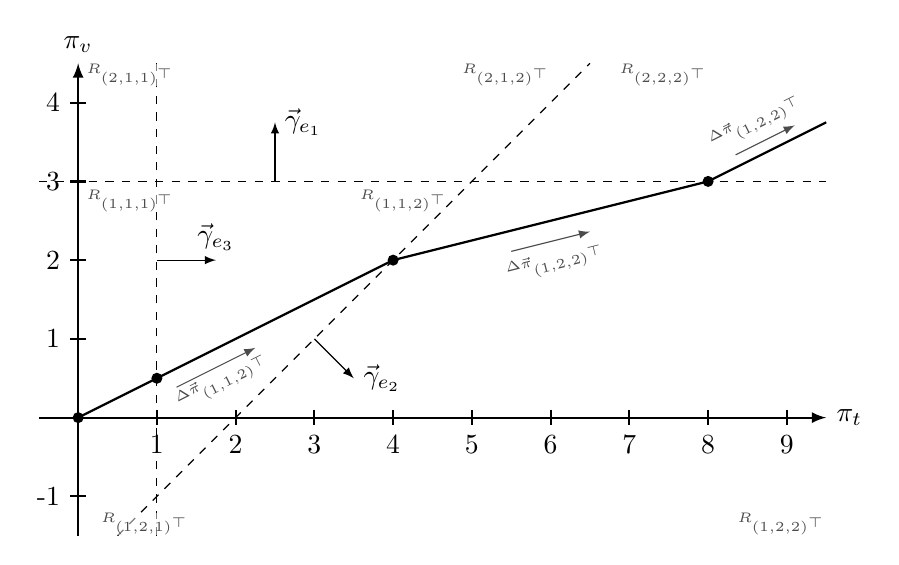
\begin{tikzpicture}
	% IMAGE SIZE
	\newcommand{\xMin}{-0.5} \newcommand{\xMax}{9.5}
	\newcommand{\yMin}{-1.5} \newcommand{\yMax}{4.5}
	
	% x-Axis
	\draw[thick, ->] (\xMin,0) -- (\xMax,0) node[anchor=west] {$\pi_t$};
	\foreach \i in {1,...,9}
	{
		\draw[thick] (\i, 0.1) -- (\i,-0.1) node[anchor=north] {\i};
	}
	%y-Axis
	\foreach \i in {-1,1,2,3,4}
	{
		\draw[thick] (0.1, \i) -- (-0.1, \i) node[anchor=east] {\i};
	}
	\draw[thick, ->] (0,\yMin) -- (0,\yMax) node[anchor=south] {$\pi_v$};
	
	%Boundaries
	\draw[dashed] (1, \yMin) -- (1, \yMax);
	\draw[dashed] (\xMin,3) -- (\xMax,3);
	\draw[dashed] ({max(\xMin,\yMin+2)},{max(\xMin-2,\yMin)}) -- ({min(\xMax,\yMax+2)},{min(\xMax-2,\yMax)});
	
	% Region labels
	\node[anchor=south east, inner sep=0pt, black!70] at (\xMax,\yMin) {\tiny $\region[(1,2,2)^{\top}]$};
	\node[anchor=north east, inner sep=0pt, black!70] at (\xMax-1.5,\yMax) {\tiny $\region[(2,2,2)^{\top}]$};
	\node[anchor=north east, inner sep=0pt, black!70] at (6,\yMax) {\tiny $\region[(2,1,2)^{\top}]$};
	\node[anchor=north west, black!70, fill=white, fill opacity=.5, text opacity=1, inner sep=0pt]
	at (0.1,\yMax) {\tiny $\region[(2,1,1)^{\top}]$};
	\node[anchor=north west, black!70, fill=white, fill opacity=.5, text opacity=1, inner sep=0pt]
	at (0.1,2.9) {\tiny $\region[(1,1,1)^{\top}]$};
	\node[anchor=north east, black!70, inner sep=0pt] at (4.7,2.9) {\tiny $\region[(1,1,2)^{\top}]$};
	\node[anchor=south, black!70, fill=white, fill opacity=.5, text opacity=1, inner sep=0pt]
	at (0.85,\yMin) {\tiny $\region[(1,2,1)^{\top}]$};
	
	
	% Normal vectors of the boundaries
	\draw[thin, ->] (2.5,3) -- (2.5, 3.75) node[right] {$\vec{\gamma}_{e_1}$};
	\draw[thin, ->] (1,2) -- (1.75, 2) node[above] {$\vec{\gamma}_{e_3}$};
	\draw[thin, ->] (3,1) -- (3.5, 0.5) node[right] {$\vec{\gamma}_{e_2}$};
	
	% Example linear function for region (1,2,2)
	%\draw[thin, black!50] ( {max(\xMin, 4*(\yMin-1))}, {max(1/4*\xMin+1, \yMin)} ) -- ( {min(\xMax, 4*(\yMax - 1))}, {min(1/4*\xMax +1, \yMax)} );
	
	%Solution Curve
	\draw[thick]
	(0,0) -- (4,2) -- (8,3) -- ++(3/2,3/4);
	
	%Solution Curve Breakpoints
	\fill (0,0) circle(2pt);
	\fill (1,1/2) circle(2pt);
	\fill (4,2) circle(2pt);
	\fill (8,3) circle(2pt);
	
	%% Potential direction example
	\draw[->, yshift=0pt, black!70, yshift=-0.75em] (1.25,.65) -- ++ (1,1/2) node[midway, below=-0.5ex, sloped] {\tiny $\potentialD[(1,1,2)^{\top}]$};
	\draw[->, yshift=0pt, black!70, yshift=-0.75em] (5.5,2+3/8) -- ++ (1,1/4) node[midway, below, sloped] {\tiny $\potentialD[(1,2,2)^{\top}]$};
	\draw[->, yshift=0pt, black!70, yshift=-0.75em] (8.35,3.6) -- ++ (3/4,3/8) node[midway, above, sloped] {\tiny $\potentialD[(1,2,2)^{\top}]$};
	\end{tikzpicture}

\end{document}